\documentclass[letterpaper,11pt,twocolumn]{article}
\usepackage[utf8]{inputenc}
\usepackage[margin=1.8cm,left=2.8cm,paper=letterpaper]{geometry}
\usepackage{amssymb, amsmath, amsfonts, latexsym}
\usepackage{graphicx, wrapfig, float, subfigure, capt-of}
\usepackage[table]{xcolor}
\usepackage{multirow, bigstrut, booktabs}
\usepackage{fancyhdr, appendix, enumerate, blindtext, makeidx}
\usepackage[spanish]{babel}
\addto\captionsspanish{
	\renewcommand{\tablename}{Tabla}
}
\usepackage[none]{hyphenat}
\usepackage[font={small}]{caption}
\usepackage[bookmarks=true, colorlinks=true, linkcolor=black, citecolor=black, menucolor=black, urlcolor=black]{hyperref}
\usepackage[backend=bibtex]{biblatex}
\usepackage{colortbl}
\usepackage{array}
\usepackage{tcolorbox}
\usepackage{minted}
\usepackage{listings}
\bibliography{referencias}

% Configuración de página
\renewcommand{\headrulewidth}{0pt}
\usepackage{color}
\definecolor{gray51}{rgb}{0.51,0.51,0.51}
\definecolor{gray71}{rgb}{0.71,0.71,0.71}

\begin{document}
	
	% === Sección de encabezado y título en una sola columna ===
	\twocolumn[{
		\begin{center}
			\begin{minipage}{0.3\textwidth}
				\centering
				
\includegraphics[width=4.5cm]{images/logo.png}
			\end{minipage}
			\hspace{0.1\textwidth}
			\begin{minipage}{0.5\textwidth}
				\centering
				\textsc{\color{red}Departamento de Ingeniería Eléctrica}\\
				\textsc{\color{gray51}Facultad de Ciencias Físicas y Matemáticas}\\
				\textsc{\color{gray51}Universidad de Chile}\\
				\textsc{\color{gray51}EL7008-1 Procesamiento Avanzado de Imágenes}
			\end{minipage}
		\end{center}
		
		\vspace{0.3cm}  % Espacio entre el encabezado y el título
		
		\begin{center}
			{\LARGE \textbf{Título}}\\
			{\Large Subtítulo}
		\end{center}
		
		\vspace{0.5cm} % Espacio entre el título y el contenido
	}]
	
	% === Contenido en dos columnas ===
	\section{Sección}
\subsection{Subsección}
\subsubsection{Subsubsección}

Rick astley \ref{fig:Rick1} and Ricks Astleys \ref{fig:Rick2}.
\begin{figure}[H]
    \centering
    \captionsetup{justification=centering}
    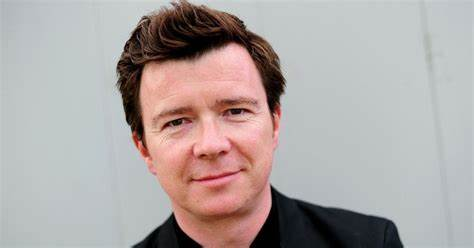
\includegraphics[width=6cm]{images/rick.jpg}
    \caption{Rick.}
    \label{fig:Rick1}
\end{figure}

\begin{figure}[H]
    \centering
    \captionsetup{justification=centering,margin=2cm}
    \subfigure[Rick.]{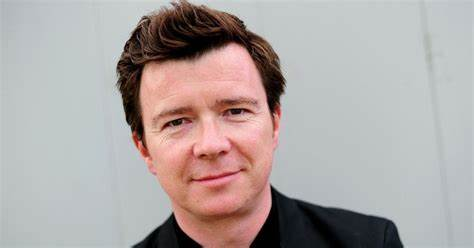
\includegraphics[width=6cm]{images/rick.jpg}}
    \subfigure[Rick.]{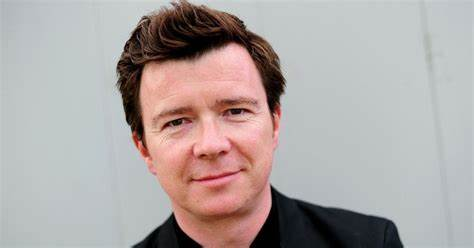
\includegraphics[width=6cm]{images/rick.jpg}}
    \subfigure[Rick.]{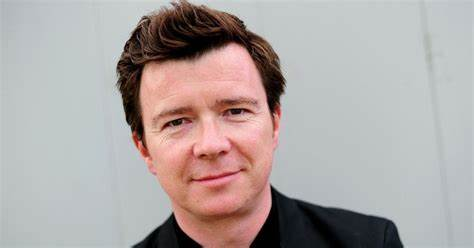
\includegraphics[width=6cm]{images/rick.jpg}}
    \subfigure[Rick.]{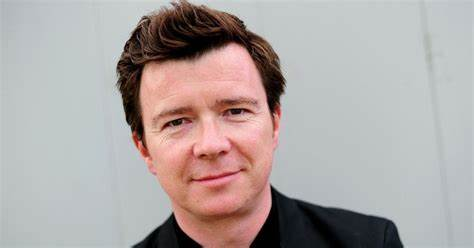
\includegraphics[width=6cm]{images/rick.jpg}}
    \caption{Rick.}
    \label{fig:Rick2}
\end{figure}

Rick cite \cite{book} and Rick cite \cite{online}
\clearpage
%%%%%%%%%%%%%%%%%%%%%%%%%%%%%%%%%%
\subsection{Sección 2}
\begin{tcolorbox}
[colback=white!5!white,colframe=green!75!black,fonttitle=\bfseries,title=Cuadro]
Había una vez truz
\end{tcolorbox}

\begin{tcolorbox}
[colback=white!5!white,colframe=blue!75!black,fonttitle=\bfseries,title=Cuadro con código]
\begin{minted}[tabsize=2,breaklines, fontsize=\scriptsize, linenos = False]{python}
def suma(a, b):
    """
    Esta función toma dos números como entrada y devuelve la suma de ellos.
    
    Args:
    a (float o int): El primer número.
    b (float o int): El segundo número.
    
    Returns:
    float o int: La suma de los dos números.
    """
    resultado = a + b
    return resultado

# Ejemplo de uso de la función
num1 = 5
num2 = 7
resultado_suma = suma(num1, num2)
print("El resultado de la suma es:", resultado_suma)

\end{minted}
\end{tcolorbox}





\href{https://youtu.be/mCdA4bJAGGk}{Texto con Hipervínculo.}


\clearpage
	\printbibliography
	
\end{document}
